\documentclass[]{article}
\usepackage{lmodern}
\usepackage{amssymb,amsmath}
\usepackage{ifxetex,ifluatex}
\usepackage{fixltx2e} % provides \textsubscript
\ifnum 0\ifxetex 1\fi\ifluatex 1\fi=0 % if pdftex
  \usepackage[T1]{fontenc}
  \usepackage[utf8]{inputenc}
\else % if luatex or xelatex
  \ifxetex
    \usepackage{mathspec}
  \else
    \usepackage{fontspec}
  \fi
  \defaultfontfeatures{Ligatures=TeX,Scale=MatchLowercase}
\fi
% use upquote if available, for straight quotes in verbatim environments
\IfFileExists{upquote.sty}{\usepackage{upquote}}{}
% use microtype if available
\IfFileExists{microtype.sty}{%
\usepackage{microtype}
\UseMicrotypeSet[protrusion]{basicmath} % disable protrusion for tt fonts
}{}
\usepackage[margin=1in]{geometry}
\usepackage{hyperref}
\hypersetup{unicode=true,
            pdftitle={Laborator 3},
            pdfborder={0 0 0},
            breaklinks=true}
\urlstyle{same}  % don't use monospace font for urls
\usepackage{color}
\usepackage{fancyvrb}
\newcommand{\VerbBar}{|}
\newcommand{\VERB}{\Verb[commandchars=\\\{\}]}
\DefineVerbatimEnvironment{Highlighting}{Verbatim}{commandchars=\\\{\}}
% Add ',fontsize=\small' for more characters per line
\usepackage{framed}
\definecolor{shadecolor}{RGB}{248,248,248}
\newenvironment{Shaded}{\begin{snugshade}}{\end{snugshade}}
\newcommand{\KeywordTok}[1]{\textcolor[rgb]{0.13,0.29,0.53}{\textbf{#1}}}
\newcommand{\DataTypeTok}[1]{\textcolor[rgb]{0.13,0.29,0.53}{#1}}
\newcommand{\DecValTok}[1]{\textcolor[rgb]{0.00,0.00,0.81}{#1}}
\newcommand{\BaseNTok}[1]{\textcolor[rgb]{0.00,0.00,0.81}{#1}}
\newcommand{\FloatTok}[1]{\textcolor[rgb]{0.00,0.00,0.81}{#1}}
\newcommand{\ConstantTok}[1]{\textcolor[rgb]{0.00,0.00,0.00}{#1}}
\newcommand{\CharTok}[1]{\textcolor[rgb]{0.31,0.60,0.02}{#1}}
\newcommand{\SpecialCharTok}[1]{\textcolor[rgb]{0.00,0.00,0.00}{#1}}
\newcommand{\StringTok}[1]{\textcolor[rgb]{0.31,0.60,0.02}{#1}}
\newcommand{\VerbatimStringTok}[1]{\textcolor[rgb]{0.31,0.60,0.02}{#1}}
\newcommand{\SpecialStringTok}[1]{\textcolor[rgb]{0.31,0.60,0.02}{#1}}
\newcommand{\ImportTok}[1]{#1}
\newcommand{\CommentTok}[1]{\textcolor[rgb]{0.56,0.35,0.01}{\textit{#1}}}
\newcommand{\DocumentationTok}[1]{\textcolor[rgb]{0.56,0.35,0.01}{\textbf{\textit{#1}}}}
\newcommand{\AnnotationTok}[1]{\textcolor[rgb]{0.56,0.35,0.01}{\textbf{\textit{#1}}}}
\newcommand{\CommentVarTok}[1]{\textcolor[rgb]{0.56,0.35,0.01}{\textbf{\textit{#1}}}}
\newcommand{\OtherTok}[1]{\textcolor[rgb]{0.56,0.35,0.01}{#1}}
\newcommand{\FunctionTok}[1]{\textcolor[rgb]{0.00,0.00,0.00}{#1}}
\newcommand{\VariableTok}[1]{\textcolor[rgb]{0.00,0.00,0.00}{#1}}
\newcommand{\ControlFlowTok}[1]{\textcolor[rgb]{0.13,0.29,0.53}{\textbf{#1}}}
\newcommand{\OperatorTok}[1]{\textcolor[rgb]{0.81,0.36,0.00}{\textbf{#1}}}
\newcommand{\BuiltInTok}[1]{#1}
\newcommand{\ExtensionTok}[1]{#1}
\newcommand{\PreprocessorTok}[1]{\textcolor[rgb]{0.56,0.35,0.01}{\textit{#1}}}
\newcommand{\AttributeTok}[1]{\textcolor[rgb]{0.77,0.63,0.00}{#1}}
\newcommand{\RegionMarkerTok}[1]{#1}
\newcommand{\InformationTok}[1]{\textcolor[rgb]{0.56,0.35,0.01}{\textbf{\textit{#1}}}}
\newcommand{\WarningTok}[1]{\textcolor[rgb]{0.56,0.35,0.01}{\textbf{\textit{#1}}}}
\newcommand{\AlertTok}[1]{\textcolor[rgb]{0.94,0.16,0.16}{#1}}
\newcommand{\ErrorTok}[1]{\textcolor[rgb]{0.64,0.00,0.00}{\textbf{#1}}}
\newcommand{\NormalTok}[1]{#1}
\usepackage{graphicx,grffile}
\makeatletter
\def\maxwidth{\ifdim\Gin@nat@width>\linewidth\linewidth\else\Gin@nat@width\fi}
\def\maxheight{\ifdim\Gin@nat@height>\textheight\textheight\else\Gin@nat@height\fi}
\makeatother
% Scale images if necessary, so that they will not overflow the page
% margins by default, and it is still possible to overwrite the defaults
% using explicit options in \includegraphics[width, height, ...]{}
\setkeys{Gin}{width=\maxwidth,height=\maxheight,keepaspectratio}
\IfFileExists{parskip.sty}{%
\usepackage{parskip}
}{% else
\setlength{\parindent}{0pt}
\setlength{\parskip}{6pt plus 2pt minus 1pt}
}
\setlength{\emergencystretch}{3em}  % prevent overfull lines
\providecommand{\tightlist}{%
  \setlength{\itemsep}{0pt}\setlength{\parskip}{0pt}}
\setcounter{secnumdepth}{5}
% Redefines (sub)paragraphs to behave more like sections
\ifx\paragraph\undefined\else
\let\oldparagraph\paragraph
\renewcommand{\paragraph}[1]{\oldparagraph{#1}\mbox{}}
\fi
\ifx\subparagraph\undefined\else
\let\oldsubparagraph\subparagraph
\renewcommand{\subparagraph}[1]{\oldsubparagraph{#1}\mbox{}}
\fi

%%% Use protect on footnotes to avoid problems with footnotes in titles
\let\rmarkdownfootnote\footnote%
\def\footnote{\protect\rmarkdownfootnote}

%%% Change title format to be more compact
\usepackage{titling}

% Create subtitle command for use in maketitle
\newcommand{\subtitle}[1]{
  \posttitle{
    \begin{center}\large#1\end{center}
    }
}

\setlength{\droptitle}{-2em}
  \title{Laborator 3}
  \pretitle{\vspace{\droptitle}\centering\huge}
  \posttitle{\par}
\subtitle{Elemente de statistică descriptivă}
  \author{}
  \preauthor{}\postauthor{}
  \date{}
  \predate{}\postdate{}

\usepackage{booktabs}
\usepackage{longtable}
\usepackage{framed,color}
\definecolor{shadecolor}{RGB}{248, 248, 248}
%\definecolor{shadecolor1}{RGB}{216,225,235}
%\definecolor{framecolor}{RGB}{108,123,13}

%\definecolor{shadecolor}{RGB}{226, 255, 241}
\definecolor{shadecolor1}{RGB}{217,225,199}
\definecolor{framecolor}{RGB}{60,179,113}

\ifxetex
  \usepackage{letltxmacro}
  \setlength{\XeTeXLinkMargin}{1pt}
  \LetLtxMacro\SavedIncludeGraphics\includegraphics
  \def\includegraphics#1#{% #1 catches optional stuff (star/opt. arg.)
    \IncludeGraphicsAux{#1}%
  }%
  \newcommand*{\IncludeGraphicsAux}[2]{%
    \XeTeXLinkBox{%
      \SavedIncludeGraphics#1{#2}%
    }%
  }%
\fi

\newenvironment{frshaded*}{%
  \def\FrameCommand{\fboxrule=\FrameRule\fboxsep=\FrameSep \fcolorbox{framecolor}{shadecolor1}}%
  \MakeFramed {\advance\hsize-\width \FrameRestore}}%
{\endMakeFramed}

\newenvironment{rmdblock}[1]
  {\begin{frshaded*}
  \begin{itemize}
  \renewcommand{\labelitemi}{
    \raisebox{-.7\height}[0pt][0pt]{
      {\setkeys{Gin}{width=2em,keepaspectratio}\includegraphics{images/icons/#1}}
    }
  }
  \item
  }
  {
  \end{itemize}
  \end{frshaded*}
  }

\newenvironment{rmdcaution}
  {\begin{rmdblock}{caution}}
  {\end{rmdblock}}
% \newenvironment{rmdinsight}
%   {\begin{rmdblock}{insight}}
%   {\end{rmdblock}}
\newenvironment{rmdexercise}
  {\begin{rmdblock}{exercise}}
  {\end{rmdblock}}
\newenvironment{rmdtip}
  {\begin{rmdblock}{tip}}
  {\end{rmdblock}}


%%%%%%%%%%%%%%%%%%%%%%%%%%%%%%%%%%%%%%%%%%%%%%%%%%%%%%%%%%%%%%%%%%%%%%%%%%%%%%%%%%%%%%%%%%%%%%%%%%%%%%%%%%%%%%%%%%%%%
%%%%%%%%%%% For insight block %%%%%%%%%%%%%%%%%%%%%%%%%%
\definecolor{shadecolor_insight}{RGB}{223,240,216}
\definecolor{framecolor_insight}{RGB}{136,193,137}

%\definecolor{shadecolor_insight}{RGB}{217,225,199}
%\definecolor{framecolor_insight}{RGB}{60,179,113}

\newenvironment{frshaded_insight*}{%
  \def\FrameCommand{\fboxrule=\FrameRule\fboxsep=\FrameSep \fcolorbox{framecolor_insight}{shadecolor_insight}}%
  \MakeFramed {\advance\hsize-\width \FrameRestore}}%
{\endMakeFramed}

\newenvironment{rmdblock_insight}[1]
  {\begin{frshaded_insight*}
  \begin{itemize}
  \renewcommand{\labelitemi}{
    \raisebox{-.7\height}[0pt][0pt]{
      {\setkeys{Gin}{width=2em,keepaspectratio}\includegraphics{images/icons/#1}}
    }
  }
  \item
  }
  {
  \end{itemize}
  \end{frshaded_insight*}
  }

\newenvironment{rmdinsight}
  {\begin{rmdblock_insight}{insight}}
  {\end{rmdblock_insight}}

%%%%%%%%%%%%%%%%%%%%%%%%%%%%%%%%%%%%%%%%%%%%%%%%%%%%%%%%%%%%%%%%%%%%%%%%%%%%%%%%%%%%%%%%%%%%%%%%%%%%%%%%%%%%%%%%%%%%%
\usepackage{subfigure}
\usepackage{booktabs}
\usepackage{slashbox}
\usepackage{color}
%%%%%%%%%%%%%%%%%%%%%%%%%%%%%%%%%%%%%%%%%%%%%%%%%%%%%%%%%%%%%%%%%%%%%%%%%%%%%%%%%%%%%%%%%%%%%%%%%%%%%%%%%%%%%%%%%%%%%
%CITEVA DEFINITII
\def\om{\omega}
\def\Om{\Omega}
\def\et{\eta}
\def\td{\tilde{\delta}}
\def\m{{\mu}}
\def\n{{\nu}}
\def\k{{\kappa}}
\def\l{{\lambda}}
\def\L{{\Lambda}}
\def\g{{\gamma}}
\def\a{{\alpha}}
\def\e{{\varepsilon}}
\def\b{{\beta}}
\def\G{{\Gamma}}
\def\d{{\delta}}
\def\D{{\Delta}}
\def\t{{\theta}}
\def\s{{\sigma}}
\def\S{{\Sigma}}
\def\z{{\zeta}}
\def\qed{\hfill\Box}
\def\ds{\displaystyle}
\def\mc{\mathcal}
%%%%%%%%%%%%%%%%%%%%%%%%%%%%%%%%%%%%%%%%%%%%%%%%%%%%%%%%%%%%%%%%%%%%%%%%%%%%%%%%%%%%%%%%%%%%%%%%%%%%%%%%%%%%%%%%%%%%%%
\def\1{{\mathbf 1}}
\def\CC{{\mathbb C}}
\def\VV{{\mathbb V}}
\def\RR{{\mathbb R}}
\def\QQ{{\mathbb Q}}
\def\ZZ{{\mathbb Z}}
\def\PP{{\mathbb P}}
\def\EE{{\mathbb E}}
\def\NN{{\mathbb N}}
\def\FF{{\mathbb F}}
%\def\SS{{\mathbb S}}
\def\MA{{\mathcal A}}
\def\MO{{\mathcal O}}
\def\MF{{\mathcal F}}
\def\ME{{\mathcal E}}
\def\MR{{\mathcal R}}
\def\MB{{\mathcal B}}
\def\MM{{\mathcal M}}
\def\MN{{\mathcal N}}
\def\MU{{\mathcal U}}
\def\MP{{\mathcal P}}
\def\MS{{\mathcal S}}
\def\MBS{{\mathbf S}}
\def\MX{{\bm{ \mathscr X}}}

% independent sign
\newcommand\independent{\protect\mathpalette{\protect\independenT}{\perp}}
\def\independenT#1#2{\mathrel{\rlap{$#1#2$}\mkern2mu{#1#2}}}

\renewcommand\tablename{Tab.}
\renewcommand{\figurename}{Fig.}

%%%%%%%%%%%%%%%%%%%%%%%%%%%%%%%%%%%%%%%%%%%%%%%%%%%%%%%%%%%%%%%%%%%%%%%%%%%%%%%%%%%%%%%%%%%%%%%%%%%%%%%%%%%%%%%%%%%%%
%Header and Footer
\usepackage{fancyhdr}

\pagestyle{fancy}
\fancyhf{}
\rhead{Universitatea din Bucure\c sti\\ Facultatea de Matematic\u a \c si Informatic\u a}
\lhead{\textit{Curs}: Instrumente Statistice pentru Finan\c te\\ \textit{Instructor}: A. Am\u arioarei}
\rfoot{Pagina \thepage}
\lfoot{Grupa: 403}
%%%%%%%%%%%%%%%%%%%%%%%%%%%%%%%%%%%%%%%
\usepackage{booktabs}
\usepackage{longtable}
\usepackage{array}
\usepackage{multirow}
\usepackage[table]{xcolor}
\usepackage{wrapfig}
\usepackage{float}
\usepackage{colortbl}
\usepackage{pdflscape}
\usepackage{tabu}
\usepackage{threeparttable}
\usepackage[normalem]{ulem}

\begin{document}
\maketitle

%%%%%%%%%%%%%%%%%%%%%%%%
\thispagestyle{fancy}

Obiectivul acestui laborator este de a prezenta câteva elemente
(numerice și grafice) de statistică descriptivă/exploratorie pentru
studiul rentabilității zilnice (\emph{daily returns}) a unui număr de
active reprezentative (assets).

\section{Importarea datelor}\label{importarea-datelor}

Înainte de a analiza datele trebuie să le descărcăm și să le punem
într-un format ușor de utilizat pentru analiză. Datele pot fi obținute
de pe diferite platforme online precum
\href{https://finance.yahoo.com/}{Yahoo!Finance} sau
\href{https://finance.google.com/finance}{Google Finance}. Mai jos este
ilustrat codul funcției \texttt{google\_stocks} care permite extragerea
datelor de pe platforma \href{https://finance.google.com/finance}{Google
Finance}:

\begin{Shaded}
\begin{Highlighting}[]
\NormalTok{google_stocks <-}\StringTok{ }\ControlFlowTok{function}\NormalTok{(sym, }\DataTypeTok{current =} \OtherTok{TRUE}\NormalTok{, }\DataTypeTok{sy =} \DecValTok{2007}\NormalTok{, }\DataTypeTok{sm =} \DecValTok{1}\NormalTok{, }\DataTypeTok{sd =} \DecValTok{1}\NormalTok{, ey, em, ed)}
\NormalTok{\{}
  \CommentTok{# sy, sm, sd, ey, em, ed corespund la}
  \CommentTok{# start year, start month, start day, end year, end month, si end day}
  
  \CommentTok{# Daca este TRUE folosim data curenta}
  \ControlFlowTok{if}\NormalTok{(current)\{}
\NormalTok{    system_time <-}\StringTok{ }\KeywordTok{as.character}\NormalTok{(}\KeywordTok{Sys.time}\NormalTok{())}
\NormalTok{    ey <-}\StringTok{ }\KeywordTok{as.numeric}\NormalTok{(}\KeywordTok{substr}\NormalTok{(system_time, }\DataTypeTok{start =} \DecValTok{1}\NormalTok{, }\DataTypeTok{stop =} \DecValTok{4}\NormalTok{))}
\NormalTok{    em <-}\StringTok{ }\KeywordTok{as.numeric}\NormalTok{(}\KeywordTok{substr}\NormalTok{(system_time, }\DataTypeTok{start =} \DecValTok{6}\NormalTok{, }\DataTypeTok{stop =} \DecValTok{7}\NormalTok{))}
\NormalTok{    ed <-}\StringTok{ }\KeywordTok{as.numeric}\NormalTok{(}\KeywordTok{substr}\NormalTok{(system_time, }\DataTypeTok{start =} \DecValTok{9}\NormalTok{, }\DataTypeTok{stop =} \DecValTok{10}\NormalTok{))}
\NormalTok{  \}}

\NormalTok{  tmp <-}\StringTok{ }\KeywordTok{tempfile}\NormalTok{()}
  
  \CommentTok{# cat("downloading ", sym, ".....\textbackslash{}n\textbackslash{}n")}
\NormalTok{  google.URL =}\StringTok{ "http://finance.google.com/finance/historical?"}
  \KeywordTok{download.file}\NormalTok{(}\KeywordTok{paste}\NormalTok{(google.URL, }\StringTok{"q="}\NormalTok{, sym, }\StringTok{"&startdate="}\NormalTok{, }
\NormalTok{                      month.abb[sm], }\StringTok{"+"}\NormalTok{, }\KeywordTok{sprintf}\NormalTok{(}\StringTok{"%.2d"}\NormalTok{, sd), }
                      \StringTok{",+"}\NormalTok{, sy, }\StringTok{"&enddate="}\NormalTok{, month.abb[em], }\StringTok{"+"}\NormalTok{, }
                      \KeywordTok{sprintf}\NormalTok{(}\StringTok{"%.2d"}\NormalTok{, ed), }\StringTok{",+"}\NormalTok{, ey, }\StringTok{"&output=csv"}\NormalTok{, }
                      \DataTypeTok{sep =} \StringTok{""}\NormalTok{), }\DataTypeTok{destfile =}\NormalTok{ tmp, }\DataTypeTok{quiet =} \OtherTok{FALSE}\NormalTok{)}
\NormalTok{  google_out <-}\StringTok{ }\KeywordTok{read.csv}\NormalTok{(tmp)}

  \CommentTok{# Redenumim prima coloana}
  \ControlFlowTok{if}\NormalTok{(}\OperatorTok{!}\KeywordTok{is.null}\NormalTok{(google_out))\{}
    \KeywordTok{names}\NormalTok{(google_out)[}\DecValTok{1}\NormalTok{] =}\StringTok{ "Date"}
\NormalTok{  \}}
  
  \CommentTok{# transformam coloana timp }
\NormalTok{  google_out}\OperatorTok{$}\NormalTok{Date =}\StringTok{ }\KeywordTok{as.Date}\NormalTok{(}\KeywordTok{strptime}\NormalTok{(google_out}\OperatorTok{$}\NormalTok{Date, }\StringTok{"%d-%B-%y"}\NormalTok{), }
                            \DataTypeTok{origin =} \StringTok{"1970-01-01"}\NormalTok{)}
  
\NormalTok{  google_out =}\StringTok{ }\NormalTok{google_out[}\KeywordTok{order}\NormalTok{(google_out}\OperatorTok{$}\NormalTok{Date), ]}
  
  \KeywordTok{return}\NormalTok{(google_out)}
\NormalTok{\}}
\end{Highlighting}
\end{Shaded}

Pachetul R,
\href{https://cran.r-project.org/web/packages/quantmod/index.html}{quantmod}
pune la dispoziție o serie de funcții care permit atât accesul la datele
din \href{https://finance.yahoo.com/}{Yahoo!Finance} sau
\href{https://finance.google.com/finance}{Google Finance}, dar și din
alte surse, cât și utilizarea unor tehnici specifice modelării
financiare. De exemplu, funcția de mai sus are echivalentul (mult mai
complez) \texttt{getSymbols()} din pachetul \emph{quantmod}.

Să presupunem că suntem interesați de stoc-urile (\emph{stock}) firmelor
Apple, Microsoft și Google din perioada \texttt{01-01-2000} până în
prezent. Pentru a extrage aceste date va trebui să folosim
simbolul/abrevierea
(\href{https://en.wikipedia.org/wiki/Ticker_symbol}{ticker symbol} -
search pe Goole după \emph{ticker symbol}) fiecărei firme separat. Vom
accesa aceste date cu ajutorul funcției \texttt{google\_stocks}:

\begin{Shaded}
\begin{Highlighting}[]
\CommentTok{# data de start}
\NormalTok{sy =}\StringTok{ }\DecValTok{2005}
\NormalTok{sm =}\StringTok{ }\DecValTok{1}
\NormalTok{sd =}\StringTok{ }\DecValTok{1}

\CommentTok{# datele}
\NormalTok{apple_data =}\StringTok{ }\KeywordTok{google_stocks}\NormalTok{(}\StringTok{"AAPL"}\NormalTok{, }\DataTypeTok{sy =}\NormalTok{ sy, }\DataTypeTok{sm =}\NormalTok{ sm, }\DataTypeTok{sd =}\NormalTok{ sd)}
\NormalTok{msft_data =}\StringTok{ }\KeywordTok{google_stocks}\NormalTok{(}\StringTok{"MSFT"}\NormalTok{, }\DataTypeTok{sy =}\NormalTok{ sy, }\DataTypeTok{sm =}\NormalTok{ sm, }\DataTypeTok{sd =}\NormalTok{ sd)}
\NormalTok{google_data =}\StringTok{ }\KeywordTok{google_stocks}\NormalTok{(}\StringTok{"GOOG"}\NormalTok{, }\DataTypeTok{sy =}\NormalTok{ sy, }\DataTypeTok{sm =}\NormalTok{ sm, }\DataTypeTok{sd =}\NormalTok{ sd)}
\end{Highlighting}
\end{Shaded}

sau citind din fisier

\begin{Shaded}
\begin{Highlighting}[]
\CommentTok{# Google data}
\NormalTok{google_data =}\StringTok{ }\KeywordTok{read.csv}\NormalTok{(}\StringTok{"dataIn/google_data.csv"}\NormalTok{, }
                       \DataTypeTok{col.names =} \KeywordTok{c}\NormalTok{(}\StringTok{"Date"}\NormalTok{, }\StringTok{"Open"}\NormalTok{, }\StringTok{"High"}\NormalTok{, }\StringTok{"Low"}\NormalTok{,}
                                     \StringTok{"Close"}\NormalTok{, }\StringTok{"Volume"}\NormalTok{, }\StringTok{"Adjusted"}\NormalTok{))}

\NormalTok{google_data}\OperatorTok{$}\NormalTok{Date =}\StringTok{ }\KeywordTok{as.Date}\NormalTok{(}\KeywordTok{strptime}\NormalTok{(}\KeywordTok{as.character}\NormalTok{(google_data}\OperatorTok{$}\NormalTok{Date), }\StringTok{"%Y-%m-%d"}\NormalTok{), }
                            \DataTypeTok{origin =} \StringTok{"1970-01-01"}\NormalTok{)}
  
\NormalTok{google_data =}\StringTok{ }\NormalTok{google_data[}\KeywordTok{order}\NormalTok{(google_data}\OperatorTok{$}\NormalTok{Date), ]}

\CommentTok{# Apple data}
\NormalTok{apple_data =}\StringTok{ }\KeywordTok{read.csv}\NormalTok{(}\StringTok{"dataIn/apple_data.csv"}\NormalTok{,}
                      \DataTypeTok{col.names =} \KeywordTok{c}\NormalTok{(}\StringTok{"Date"}\NormalTok{, }\StringTok{"Open"}\NormalTok{, }\StringTok{"High"}\NormalTok{, }\StringTok{"Low"}\NormalTok{,}
                                     \StringTok{"Close"}\NormalTok{, }\StringTok{"Volume"}\NormalTok{, }\StringTok{"Adjusted"}\NormalTok{))}
\NormalTok{apple_data}\OperatorTok{$}\NormalTok{Date =}\StringTok{ }\KeywordTok{as.Date}\NormalTok{(}\KeywordTok{strptime}\NormalTok{(}\KeywordTok{as.character}\NormalTok{(apple_data}\OperatorTok{$}\NormalTok{Date), }\StringTok{"%Y-%m-%d"}\NormalTok{), }
                            \DataTypeTok{origin =} \StringTok{"1970-01-01"}\NormalTok{)}
  
\NormalTok{apple_data =}\StringTok{ }\NormalTok{apple_data[}\KeywordTok{order}\NormalTok{(apple_data}\OperatorTok{$}\NormalTok{Date), ]}

\CommentTok{# Microsoft data}
\NormalTok{msft_data =}\StringTok{ }\KeywordTok{read.csv}\NormalTok{(}\StringTok{"dataIn/msft_data.csv"}\NormalTok{,}
                     \DataTypeTok{col.names =} \KeywordTok{c}\NormalTok{(}\StringTok{"Date"}\NormalTok{, }\StringTok{"Open"}\NormalTok{, }\StringTok{"High"}\NormalTok{, }\StringTok{"Low"}\NormalTok{,}
                                     \StringTok{"Close"}\NormalTok{, }\StringTok{"Volume"}\NormalTok{, }\StringTok{"Adjusted"}\NormalTok{))}

\NormalTok{msft_data}\OperatorTok{$}\NormalTok{Date =}\StringTok{ }\KeywordTok{as.Date}\NormalTok{(}\KeywordTok{strptime}\NormalTok{(}\KeywordTok{as.character}\NormalTok{(msft_data}\OperatorTok{$}\NormalTok{Date), }\StringTok{"%Y-%m-%d"}\NormalTok{), }
                            \DataTypeTok{origin =} \StringTok{"1970-01-01"}\NormalTok{)}
  
\NormalTok{msft_data =}\StringTok{ }\NormalTok{msft_data[}\KeywordTok{order}\NormalTok{(msft_data}\OperatorTok{$}\NormalTok{Date), ]}
\end{Highlighting}
\end{Shaded}

Același lucru poate fi obținut cu ajutorul funcției \texttt{getSymbols}
(descărcate de pe \href{https://finance.yahoo.com/}{Yahoo!Finance}):

\begin{Shaded}
\begin{Highlighting}[]
\CommentTok{# pt a utiliza pachetul trebuie incarcat}
\ControlFlowTok{if}\NormalTok{ (}\OperatorTok{!}\KeywordTok{require}\NormalTok{(}\StringTok{"quantmod"}\NormalTok{)) \{}
    \KeywordTok{install.packages}\NormalTok{(}\StringTok{"quantmod"}\NormalTok{)}
    \KeywordTok{library}\NormalTok{(quantmod)}
\NormalTok{\}}

\CommentTok{# data de start}
\NormalTok{start <-}\StringTok{ }\KeywordTok{as.Date}\NormalTok{(}\StringTok{"2005-01-01"}\NormalTok{)}

\CommentTok{# datele din Yahoo finance}
\NormalTok{apple_data_yh =}\StringTok{ }\KeywordTok{data.frame}\NormalTok{(}\KeywordTok{getSymbols}\NormalTok{(}\StringTok{"AAPL"}\NormalTok{, }\DataTypeTok{from =}\NormalTok{ start, }\DataTypeTok{auto.assign =}\NormalTok{ F))}
\NormalTok{msft_data_yh =}\StringTok{ }\KeywordTok{data.frame}\NormalTok{(}\KeywordTok{getSymbols}\NormalTok{(}\StringTok{"MSFT"}\NormalTok{, }\DataTypeTok{from =}\NormalTok{ start, }\DataTypeTok{auto.assign =}\NormalTok{ F))}
\NormalTok{google_data_yh =}\StringTok{ }\KeywordTok{data.frame}\NormalTok{(}\KeywordTok{getSymbols}\NormalTok{(}\StringTok{"GOOG"}\NormalTok{, }\DataTypeTok{from =}\NormalTok{ start, }\DataTypeTok{auto.assign =}\NormalTok{ F))}
\end{Highlighting}
\end{Shaded}

Vom folosi în cele ce urmează datele obținute cu funcția
\texttt{google\_stocks}.
\href{https://finance.google.com/finance}{Google Finance} oferă 5 serii
pentru fiecare bun/activ. \emph{Open} corespunde prețului stoc-ului la
începutul zilei de tranzacționare și nu trebuie să fie neapărat egal cu
prețul cu care s-a închis ziua precedentă, \emph{High} și respectiv
\emph{Low} este prețul cel mai mare și respectiv cel mai mic din ziua de
tranzacționare, iar \emph{Close} este prețul stoc-ului la închiderea
zilei de tranzacționare. Coloana \emph{Volume} arată câte stoc-uri au
fost tranzacționate în ziua respectivă.

\begin{Shaded}
\begin{Highlighting}[]
\KeywordTok{head}\NormalTok{(apple_data, }\DataTypeTok{n =} \DecValTok{5}\NormalTok{)}
\NormalTok{        Date     Open     High      Low    Close    Volume Adjusted}
\DecValTok{1} \DecValTok{2005}\OperatorTok{-}\DecValTok{01}\OperatorTok{-}\DecValTok{03} \FloatTok{4.627143} \FloatTok{4.650714} \FloatTok{4.471428} \FloatTok{4.520714} \DecValTok{172998000} \FloatTok{3.060327}
\DecValTok{2} \DecValTok{2005}\OperatorTok{-}\DecValTok{01}\OperatorTok{-}\DecValTok{04} \FloatTok{4.556428} \FloatTok{4.676429} \FloatTok{4.497857} \FloatTok{4.567143} \DecValTok{274202600} \FloatTok{3.091757}
\DecValTok{3} \DecValTok{2005}\OperatorTok{-}\DecValTok{01}\OperatorTok{-}\DecValTok{05} \FloatTok{4.604286} \FloatTok{4.660714} \FloatTok{4.575000} \FloatTok{4.607143} \DecValTok{170108400} \FloatTok{3.118836}
\DecValTok{4} \DecValTok{2005}\OperatorTok{-}\DecValTok{01}\OperatorTok{-}\DecValTok{06} \FloatTok{4.619286} \FloatTok{4.636428} \FloatTok{4.523571} \FloatTok{4.610714} \DecValTok{176388800} \FloatTok{3.121253}
\DecValTok{5} \DecValTok{2005}\OperatorTok{-}\DecValTok{01}\OperatorTok{-}\DecValTok{07} \FloatTok{4.642857} \FloatTok{4.973571} \FloatTok{4.625000} \FloatTok{4.946429} \DecValTok{556862600} \FloatTok{3.348517}
\KeywordTok{head}\NormalTok{(msft_data, }\DataTypeTok{n =} \DecValTok{5}\NormalTok{)}
\NormalTok{        Date  Open  High   Low Close    Volume Adjusted}
\DecValTok{1} \DecValTok{2005}\OperatorTok{-}\DecValTok{01}\OperatorTok{-}\DecValTok{03} \FloatTok{26.80} \FloatTok{26.95} \FloatTok{26.65} \FloatTok{26.74}  \DecValTok{65002900} \FloatTok{19.93452}
\DecValTok{2} \DecValTok{2005}\OperatorTok{-}\DecValTok{01}\OperatorTok{-}\DecValTok{04} \FloatTok{26.87} \FloatTok{27.10} \FloatTok{26.66} \FloatTok{26.84} \DecValTok{109442100} \FloatTok{20.00907}
\DecValTok{3} \DecValTok{2005}\OperatorTok{-}\DecValTok{01}\OperatorTok{-}\DecValTok{05} \FloatTok{26.84} \FloatTok{27.10} \FloatTok{26.76} \FloatTok{26.78}  \DecValTok{72463500} \FloatTok{19.96435}
\DecValTok{4} \DecValTok{2005}\OperatorTok{-}\DecValTok{01}\OperatorTok{-}\DecValTok{06} \FloatTok{26.85} \FloatTok{27.06} \FloatTok{26.64} \FloatTok{26.75}  \DecValTok{76890500} \FloatTok{19.94198}
\DecValTok{5} \DecValTok{2005}\OperatorTok{-}\DecValTok{01}\OperatorTok{-}\DecValTok{07} \FloatTok{26.82} \FloatTok{26.89} \FloatTok{26.62} \FloatTok{26.67}  \DecValTok{68723300} \FloatTok{19.88235}
\KeywordTok{head}\NormalTok{(google_data, }\DataTypeTok{n =} \DecValTok{5}\NormalTok{)}
\NormalTok{        Date      Open      High      Low     Close   Volume  Adjusted}
\DecValTok{1} \DecValTok{2005}\OperatorTok{-}\DecValTok{01}\OperatorTok{-}\DecValTok{03}  \FloatTok{98.06220} \FloatTok{101.16204} \FloatTok{97.09847} \FloatTok{100.70004} \DecValTok{31894300} \FloatTok{100.70004}
\DecValTok{2} \DecValTok{2005}\OperatorTok{-}\DecValTok{01}\OperatorTok{-}\DecValTok{04} \FloatTok{100.04928} \FloatTok{100.80933} \FloatTok{96.11487}  \FloatTok{96.62157} \DecValTok{27690700}  \FloatTok{96.62157}
\DecValTok{3} \DecValTok{2005}\OperatorTok{-}\DecValTok{01}\OperatorTok{-}\DecValTok{05}  \FloatTok{96.09996}  \FloatTok{97.81381} \FloatTok{95.49390}  \FloatTok{96.12977} \DecValTok{16580200}  \FloatTok{96.12977}
\DecValTok{4} \DecValTok{2005}\OperatorTok{-}\DecValTok{01}\OperatorTok{-}\DecValTok{06}  \FloatTok{96.90970}  \FloatTok{97.31705} \FloatTok{93.25348}  \FloatTok{93.66579} \DecValTok{20909100}  \FloatTok{93.66579}
\DecValTok{5} \DecValTok{2005}\OperatorTok{-}\DecValTok{01}\OperatorTok{-}\DecValTok{07}  \FloatTok{94.70404}  \FloatTok{96.49738} \FloatTok{93.78005}  \FloatTok{96.29867} \DecValTok{19451500}  \FloatTok{96.29867}
\end{Highlighting}
\end{Shaded}

Pentru a vizualiza evoluția prețului stoc-ului la închidere avem
următoarele grafice:

\begin{Shaded}
\begin{Highlighting}[]
\KeywordTok{plot}\NormalTok{(google_data}\OperatorTok{$}\NormalTok{Date, google_data}\OperatorTok{$}\NormalTok{Close, }
     \DataTypeTok{type =} \StringTok{"l"}\NormalTok{, }
     \DataTypeTok{col =} \StringTok{"royalblue"}\NormalTok{,}
     \DataTypeTok{bty =} \StringTok{"n"}\NormalTok{,}
     \DataTypeTok{ylim =} \KeywordTok{c}\NormalTok{(}\KeywordTok{min}\NormalTok{(}\KeywordTok{c}\NormalTok{(google_data}\OperatorTok{$}\NormalTok{Close, apple_data}\OperatorTok{$}\NormalTok{Close, msft_data}\OperatorTok{$}\NormalTok{Close), }\DataTypeTok{na.rm =} \OtherTok{TRUE}\NormalTok{),}
              \KeywordTok{max}\NormalTok{(}\KeywordTok{c}\NormalTok{(google_data}\OperatorTok{$}\NormalTok{Close, apple_data}\OperatorTok{$}\NormalTok{Close, msft_data}\OperatorTok{$}\NormalTok{Close), }\DataTypeTok{na.rm =} \OtherTok{TRUE}\NormalTok{)),}
     \DataTypeTok{xlab =} \StringTok{"Perioada"}\NormalTok{, }
     \DataTypeTok{ylab =} \StringTok{"Pretul"}\NormalTok{)}

\KeywordTok{lines}\NormalTok{(apple_data}\OperatorTok{$}\NormalTok{Date, apple_data}\OperatorTok{$}\NormalTok{Close,}
      \DataTypeTok{col =} \StringTok{"brown3"}\NormalTok{)}
\KeywordTok{lines}\NormalTok{(msft_data}\OperatorTok{$}\NormalTok{Date, msft_data}\OperatorTok{$}\NormalTok{Close, }
      \DataTypeTok{col =} \StringTok{"forestgreen"}\NormalTok{)}

\KeywordTok{legend}\NormalTok{(}\StringTok{"topleft"}\NormalTok{, }
       \DataTypeTok{legend =} \KeywordTok{c}\NormalTok{(}\StringTok{"Google"}\NormalTok{, }\StringTok{"Apple"}\NormalTok{, }\StringTok{"Microsoft"}\NormalTok{), }
       \DataTypeTok{col =} \KeywordTok{c}\NormalTok{(}\StringTok{"royalblue"}\NormalTok{, }\StringTok{"brown3"}\NormalTok{, }\StringTok{"forestgreen"}\NormalTok{), }
       \DataTypeTok{lty =} \DecValTok{1}\NormalTok{,}
       \DataTypeTok{bty =} \StringTok{"n"}\NormalTok{)}
\end{Highlighting}
\end{Shaded}

\begin{center}\includegraphics[width=0.8\linewidth]{Lab_3_files/figure-latex/unnamed-chunk-7-1} \end{center}

\section{Rentabilitate (Returns)}\label{rentabilitate-returns}

Scopul unei investiții este acela de a face profit, prin urmare
investitorii sunt interesași în a face investiții care produc venituri
mari relativ la mărimea investiției. Rentabilitatea / Rata de
rentabilitate (returns) măsoară modificarea prețului unui bun exprimat
ca o fracție din prețul inițial.

\subsection{Rentabilitate netă și brută (net and gross
return)}\label{rentabilitate-neta-si-bruta-net-and-gross-return}

Să presupunem că achiziționăm un bun (activ, stock, etc.) la momentul
\(t_0\) cu prețul \(P_{t_0}\) și îl vindem la momentul \(t_1\) cu prețul
\(P_{t_1}\). Dacă între \(t_0\) și \(t_1\) nu avem schimbări de preț
atunci rata de rentabilitate pe perioada \(t_0\) - \(t_1\) este

\[
  R(t_0,t_1) = \frac{P_{t_1} - P_{t_0}}{P_{t_0}}.
\]

Perioada dintre \(t_0\) și \(t_1\) se numește perioada de retenție a
bunului (\emph{holding period}), perioada dintre achiziția și vânzarea
unui bun (activ, etc.), și poate fi măsurată în secunde, minute, ore,
zile, luni, etc. Dacă \(P_t\) este prețul unui activ la momentul \(t\)
(să zicem la sfârșitul lunii \(t\)) și \(P_{t-1}\) este prețul activului
la momentul \(t-1\) atunci rentabilitatea netă (\emph{net return}) în
perioada de la \(t-1\) la \(t\) este

\[
  R_t = \frac{P_{t} - P_{t-1}}{P_{t-1}}
\]

și putem spune că

\[
  \text{venitul } = \text{ investitia initiala } \times \text{ rentabilitatea neta}.
\]

Rentabilitatea brută (\emph{gross return}) este definită prin

\[
  \frac{P_{t}}{P_{t-1}} = 1 + R_t.
\]

Spre exemplu să considerăm o investiție de o lună într-un stock
Microsoft. Să presupunem că achiziționăm stock-ul în luna \(t-1\) cu
prețul \(P_{t-1} = 85\, u.m.\) și îl vindem în luna următoare cu
\(P_{t} = 90\, u.m.\). Atunci rentabilitatea netă și brută pe perioada
de 1 lună sunt: \(R_t = \frac{90-85}{85} = 0.058\) iar \(1+R_t = 1.058\)
ceea ce înseamnă că investiția a condus la o rentabiltate de \(5.8\%\)
sau altfel spus \(1\,u.m.\) investită în stock-ul Microsoft în luna
\(t-1\) a crescut la \(1.058\,u.m.\) în luna \(t\) (creșterea a fost de
\(105.8\%\)).

Să presupunem că vrem să calculăm rentabilitatea zilnică (netă și brută)
a stock-urilor Apple, Google și Microsoft:

\begin{Shaded}
\begin{Highlighting}[]
\CommentTok{# Rentabilitatea zilnica }
\NormalTok{google_ret_s_daily =}\StringTok{ }\NormalTok{google_data}\OperatorTok{$}\NormalTok{Close[}\OperatorTok{-}\DecValTok{1}\NormalTok{] }\OperatorTok{/}\StringTok{ }\NormalTok{google_data}\OperatorTok{$}\NormalTok{Close[}\OperatorTok{-}\KeywordTok{length}\NormalTok{(google_data}\OperatorTok{$}\NormalTok{Close)] }\OperatorTok{-}\StringTok{ }\DecValTok{1} 
\NormalTok{apple_ret_s_daily =}\StringTok{ }\NormalTok{apple_data}\OperatorTok{$}\NormalTok{Close[}\OperatorTok{-}\DecValTok{1}\NormalTok{] }\OperatorTok{/}\StringTok{ }\NormalTok{apple_data}\OperatorTok{$}\NormalTok{Close[}\OperatorTok{-}\KeywordTok{length}\NormalTok{(apple_data}\OperatorTok{$}\NormalTok{Close)] }\OperatorTok{-}\StringTok{ }\DecValTok{1} 
\NormalTok{msft_ret_s_daily =}\StringTok{ }\NormalTok{msft_data}\OperatorTok{$}\NormalTok{Close[}\OperatorTok{-}\DecValTok{1}\NormalTok{] }\OperatorTok{/}\StringTok{ }\NormalTok{msft_data}\OperatorTok{$}\NormalTok{Close[}\OperatorTok{-}\KeywordTok{length}\NormalTok{(msft_data}\OperatorTok{$}\NormalTok{Close)] }\OperatorTok{-}\StringTok{ }\DecValTok{1} 

\KeywordTok{head}\NormalTok{(}\KeywordTok{cbind}\NormalTok{(google_ret_s_daily, apple_ret_s_daily, msft_ret_s_daily))}
\NormalTok{     google_ret_s_daily apple_ret_s_daily msft_ret_s_daily}
\NormalTok{[}\DecValTok{1}\NormalTok{,]       }\OperatorTok{-}\FloatTok{0.040501234}      \FloatTok{0.0102702803}      \FloatTok{0.003739716}
\NormalTok{[}\DecValTok{2}\NormalTok{,]       }\OperatorTok{-}\FloatTok{0.005089951}      \FloatTok{0.0087582105}     \OperatorTok{-}\FloatTok{0.002235432}
\NormalTok{[}\DecValTok{3}\NormalTok{,]       }\OperatorTok{-}\FloatTok{0.025631748}      \FloatTok{0.0007751008}     \OperatorTok{-}\FloatTok{0.001120276}
\NormalTok{[}\DecValTok{4}\NormalTok{,]        }\FloatTok{0.028109237}      \FloatTok{0.0728119332}     \OperatorTok{-}\FloatTok{0.002990654}
\NormalTok{[}\DecValTok{5}\NormalTok{,]        }\FloatTok{0.006241924}     \OperatorTok{-}\FloatTok{0.0041878697}      \FloatTok{0.004874353}
\NormalTok{[}\DecValTok{6}\NormalTok{,]       }\OperatorTok{-}\FloatTok{0.007792465}     \OperatorTok{-}\FloatTok{0.0638049631}     \OperatorTok{-}\FloatTok{0.002611903}
\end{Highlighting}
\end{Shaded}

\begin{center}\includegraphics[width=0.8\linewidth]{Lab_3_files/figure-latex/unnamed-chunk-9-1} \end{center}

și rentabilitatea lunară:

\begin{Shaded}
\begin{Highlighting}[]
\CommentTok{# Rentabilitatea lunara}
\NormalTok{returnMonth =}\StringTok{ }\ControlFlowTok{function}\NormalTok{(dat)\{}
\NormalTok{  dat}\OperatorTok{$}\NormalTok{Day =}\StringTok{ }\KeywordTok{as.numeric}\NormalTok{(}\KeywordTok{strftime}\NormalTok{(dat}\OperatorTok{$}\NormalTok{Date, }\StringTok{"%d"}\NormalTok{))}
\NormalTok{  dat}\OperatorTok{$}\NormalTok{Month =}\StringTok{ }\KeywordTok{as.numeric}\NormalTok{(}\KeywordTok{strftime}\NormalTok{(dat}\OperatorTok{$}\NormalTok{Date, }\StringTok{"%m"}\NormalTok{))}
\NormalTok{  dat}\OperatorTok{$}\NormalTok{Year =}\StringTok{ }\KeywordTok{as.numeric}\NormalTok{(}\KeywordTok{strftime}\NormalTok{(dat}\OperatorTok{$}\NormalTok{Date, }\StringTok{"%Y"}\NormalTok{))}
  
\NormalTok{  dat_month_diff =}\StringTok{ }\KeywordTok{diff}\NormalTok{(dat}\OperatorTok{$}\NormalTok{Month)}
\NormalTok{  dat_month =}\StringTok{ }\NormalTok{dat[dat_month_diff }\OperatorTok{==}\StringTok{ }\DecValTok{1}\NormalTok{, ]}
  
\NormalTok{  month_ret =}\StringTok{ }\NormalTok{dat_month}\OperatorTok{$}\NormalTok{Close[}\OperatorTok{-}\DecValTok{1}\NormalTok{] }\OperatorTok{/}\StringTok{ }\NormalTok{dat_month}\OperatorTok{$}\NormalTok{Close[}\OperatorTok{-}\KeywordTok{length}\NormalTok{(dat_month}\OperatorTok{$}\NormalTok{Close)] }\OperatorTok{-}\StringTok{ }\DecValTok{1} 
  \KeywordTok{return}\NormalTok{(}\KeywordTok{data.frame}\NormalTok{(}\DataTypeTok{date =}\NormalTok{ dat_month}\OperatorTok{$}\NormalTok{Date[}\OperatorTok{-}\DecValTok{1}\NormalTok{], }\DataTypeTok{ret =}\NormalTok{ month_ret))}
\NormalTok{\}}

\NormalTok{google_ret_s_monthly =}\StringTok{ }\KeywordTok{returnMonth}\NormalTok{(google_data)}
\NormalTok{apple_ret_s_monthly =}\StringTok{ }\KeywordTok{returnMonth}\NormalTok{(apple_data)}
\NormalTok{msft_ret_s_monthly =}\StringTok{ }\KeywordTok{returnMonth}\NormalTok{(msft_data)}

\KeywordTok{head}\NormalTok{(}\KeywordTok{cbind}\NormalTok{(google_ret_s_monthly}\OperatorTok{$}\NormalTok{ret, apple_ret_s_monthly}\OperatorTok{$}\NormalTok{ret, }
\NormalTok{           msft_ret_s_monthly}\OperatorTok{$}\NormalTok{ret))}
\NormalTok{            [,}\DecValTok{1}\NormalTok{]        [,}\DecValTok{2}\NormalTok{]        [,}\DecValTok{3}\NormalTok{]}
\NormalTok{[}\DecValTok{1}\NormalTok{,] }\OperatorTok{-}\FloatTok{0.03900416}  \FloatTok{0.16670997} \OperatorTok{-}\FloatTok{0.04261800}
\NormalTok{[}\DecValTok{2}\NormalTok{,] }\OperatorTok{-}\FloatTok{0.03978939} \OperatorTok{-}\FloatTok{0.07111008} \OperatorTok{-}\FloatTok{0.03934817}
\NormalTok{[}\DecValTok{3}\NormalTok{,]  }\FloatTok{0.21876907} \OperatorTok{-}\FloatTok{0.13462914}  \FloatTok{0.04675213}
\NormalTok{[}\DecValTok{4}\NormalTok{,]  }\FloatTok{0.26031817}  \FloatTok{0.10260667}  \FloatTok{0.01976285}
\NormalTok{[}\DecValTok{5}\NormalTok{,]  }\FloatTok{0.06087933} \OperatorTok{-}\FloatTok{0.07419507} \OperatorTok{-}\FloatTok{0.03720927}
\NormalTok{[}\DecValTok{6}\NormalTok{,] }\OperatorTok{-}\FloatTok{0.02172367}  \FloatTok{0.15865239}  \FloatTok{0.03099843}
\end{Highlighting}
\end{Shaded}

\begin{center}\includegraphics[width=0.8\linewidth]{Lab_3_files/figure-latex/unnamed-chunk-11-1} \end{center}

Rentabilitatea brută pe o \(k\)-perioadă (dacă \(k=2\) și perioada este
o lună atunci avem rentabilitatea brută pentru 2 luni) este dată de
formula

\[
  1+R_{t}(k) = \frac{P_t}{P_{t-k}} = \frac{P_{t}}{P_{t-1}}\frac{P_{t-1}}{P_{t-2}}\cdots \frac{P_{t-k+1}}{P_{t-k}} = \prod_{j=0}^{k-1}(1+R_{t-j}).
\]

\subsection{Rentabilitate compusă / logaritmică (log
returns)}\label{rentabilitate-compusa-logaritmica-log-returns}

Dacă luăm prețurile în scară logaritmică, \(p_t = \log(P_t)\), atunci
definim logaritmul rentabilității - \emph{log returns} (sau
\emph{continuously compounded returns}) prin

\[
  r_t = \log(1+R_t) = p_t-p_{t-1}.
\]

Deoarece, pentru \(x\) suficient de mic putem folosi aproximarea
\(\log(1+x)\approx x\), putem spune că \(r_t\approx R_t\) în special
pentru rentabilități calculate pe perioade scurte de timp
(e.g.~zilnice).

\begin{center}\includegraphics[width=0.8\linewidth]{Lab_3_files/figure-latex/unnamed-chunk-12-1} \end{center}

De asemenea avem că

\[
  r_t(k) = \log(1+R_t(k)) = \log\left(\prod_{j=0}^{k-1}(1+R_{t-j})\right) = \sum_{j = 0}^{k-1}r_{t-j}.
\]

Pentru datele noastre avem

\begin{Shaded}
\begin{Highlighting}[]
\CommentTok{# log returns }
\NormalTok{google_ret_s_monthly}\OperatorTok{$}\NormalTok{cret =}\StringTok{ }\KeywordTok{log}\NormalTok{(}\DecValTok{1}\OperatorTok{+}\NormalTok{google_ret_s_monthly}\OperatorTok{$}\NormalTok{ret)}
\NormalTok{apple_ret_s_monthly}\OperatorTok{$}\NormalTok{cret =}\StringTok{ }\KeywordTok{log}\NormalTok{(}\DecValTok{1}\OperatorTok{+}\NormalTok{apple_ret_s_monthly}\OperatorTok{$}\NormalTok{ret)}
\NormalTok{msft_ret_s_monthly}\OperatorTok{$}\NormalTok{cret =}\StringTok{ }\KeywordTok{log}\NormalTok{(}\DecValTok{1}\OperatorTok{+}\NormalTok{msft_ret_s_monthly}\OperatorTok{$}\NormalTok{ret)}

\CommentTok{# ilustrare grafica}
\KeywordTok{plot}\NormalTok{(google_ret_s_monthly}\OperatorTok{$}\NormalTok{date, google_ret_s_monthly}\OperatorTok{$}\NormalTok{cret,}
     \DataTypeTok{type =} \StringTok{"l"}\NormalTok{, }
     \DataTypeTok{col =} \StringTok{"royalblue"}\NormalTok{,}
     \DataTypeTok{main =} \StringTok{"Goolge - Apple - Microsoft log returns"}\NormalTok{,}
     \DataTypeTok{xlab =} \StringTok{"Perioada (Luni)"}\NormalTok{,}
     \DataTypeTok{ylab =} \StringTok{"Log Returns"}\NormalTok{,}
     \DataTypeTok{bty =} \StringTok{"n"}\NormalTok{)}

\KeywordTok{lines}\NormalTok{(apple_ret_s_monthly}\OperatorTok{$}\NormalTok{date, apple_ret_s_monthly}\OperatorTok{$}\NormalTok{cret,}
      \DataTypeTok{col =} \StringTok{"brown3"}\NormalTok{,}
      \DataTypeTok{lty =} \DecValTok{2}\NormalTok{)}

\KeywordTok{lines}\NormalTok{(msft_ret_s_monthly}\OperatorTok{$}\NormalTok{date, msft_ret_s_monthly}\OperatorTok{$}\NormalTok{cret,}
      \DataTypeTok{col =} \StringTok{"forestgreen"}\NormalTok{,}
      \DataTypeTok{lty =} \DecValTok{3}\NormalTok{)}

\KeywordTok{legend}\NormalTok{(}\StringTok{"bottomright"}\NormalTok{, }
       \DataTypeTok{legend =} \KeywordTok{c}\NormalTok{(}\StringTok{"Google"}\NormalTok{, }\StringTok{"Apple"}\NormalTok{, }\StringTok{"Microsoft"}\NormalTok{), }
       \DataTypeTok{col =} \KeywordTok{c}\NormalTok{(}\StringTok{"royalblue"}\NormalTok{, }\StringTok{"brown3"}\NormalTok{, }\StringTok{"forestgreen"}\NormalTok{), }
       \DataTypeTok{lty =} \KeywordTok{c}\NormalTok{(}\DecValTok{1}\NormalTok{,}\DecValTok{2}\NormalTok{,}\DecValTok{3}\NormalTok{),}
       \DataTypeTok{bty =} \StringTok{"n"}\NormalTok{)}
\end{Highlighting}
\end{Shaded}

\begin{center}\includegraphics[width=0.8\linewidth]{Lab_3_files/figure-latex/unnamed-chunk-13-1} \end{center}

\subsection{Ajustarea pentru
dividende}\label{ajustarea-pentru-dividende}

Dacă un activ plătește un
\href{https://ro.wikipedia.org/wiki/Dividend}{dividend} \(D_t\) undeva
între momentul de timp \(t-1\) și \(t\) atunci rentabilitatea brută la
momentul \(t\) se calculează după formula

\[
  1+R_t = \frac{P_t+D_t}{P_{t-1}}
\] iar rentabilitatea netă este
\(R_t = \frac{P_t+D_t-P_{t-1}}{P_{t-1}} = \frac{P_t-P_{t-1}}{P_{t-1}} + \frac{D_t}{P_{t-1}}\)
unde \(\frac{P_t-P_{t-1}}{P_{t-1}}\) se numește câștigul de capital
(\emph{capital gain}) iar \(\frac{D_t}{P_{t-1}}\) se numește randamentul
dividendului (\emph{dividend yield}). Avem astfel că

\[
  1+R_{t}(k) = \prod_{j=0}^{k-1}\frac{P_{t-j}+D_{t-j}}{P_{t-j-1}} = \prod_{j=0}^{k-1}(1+R_{t-j})
\]

iar

\[
  r_t(k) = \log(1+R_t(k)) = \sum_{j=0}^{k-1}\log\left(\frac{P_{t-j}+D_{t-j}}{P_{t-j-1}}\right).
\] Pentru a calcula rentabilitățile ajustate vom folosi coloana
\texttt{Adjusted} (care apare doar la datele de pe Yahoo Finance !):

\begin{Shaded}
\begin{Highlighting}[]
\CommentTok{# Rentabilitatea lunara ajustata pentru dividende }
\NormalTok{returnMonthAdjusted =}\StringTok{ }\ControlFlowTok{function}\NormalTok{(dat)\{}
\NormalTok{  dat}\OperatorTok{$}\NormalTok{Day =}\StringTok{ }\KeywordTok{as.numeric}\NormalTok{(}\KeywordTok{strftime}\NormalTok{(dat}\OperatorTok{$}\NormalTok{Date, }\StringTok{"%d"}\NormalTok{))}
\NormalTok{  dat}\OperatorTok{$}\NormalTok{Month =}\StringTok{ }\KeywordTok{as.numeric}\NormalTok{(}\KeywordTok{strftime}\NormalTok{(dat}\OperatorTok{$}\NormalTok{Date, }\StringTok{"%m"}\NormalTok{))}
\NormalTok{  dat}\OperatorTok{$}\NormalTok{Year =}\StringTok{ }\KeywordTok{as.numeric}\NormalTok{(}\KeywordTok{strftime}\NormalTok{(dat}\OperatorTok{$}\NormalTok{Date, }\StringTok{"%Y"}\NormalTok{))}
  
\NormalTok{  dat_month_diff =}\StringTok{ }\KeywordTok{diff}\NormalTok{(dat}\OperatorTok{$}\NormalTok{Month)}
\NormalTok{  dat_month =}\StringTok{ }\NormalTok{dat[dat_month_diff }\OperatorTok{==}\StringTok{ }\DecValTok{1}\NormalTok{, ]}
  
\NormalTok{  month_ret =}\StringTok{ }\NormalTok{dat_month}\OperatorTok{$}\NormalTok{Adjusted[}\OperatorTok{-}\DecValTok{1}\NormalTok{] }\OperatorTok{/}\StringTok{ }\NormalTok{dat_month}\OperatorTok{$}\NormalTok{Adjusted[}\OperatorTok{-}\KeywordTok{length}\NormalTok{(dat_month}\OperatorTok{$}\NormalTok{Adjusted)] }\OperatorTok{-}\StringTok{ }\DecValTok{1} 
  \KeywordTok{return}\NormalTok{(}\KeywordTok{data.frame}\NormalTok{(}\DataTypeTok{date =}\NormalTok{ dat_month}\OperatorTok{$}\NormalTok{Date[}\OperatorTok{-}\DecValTok{1}\NormalTok{], }\DataTypeTok{ret =}\NormalTok{ month_ret))}
\NormalTok{\}}

\NormalTok{google_ret_adj_monthly =}\StringTok{ }\KeywordTok{returnMonthAdjusted}\NormalTok{(google_data)}
\NormalTok{apple_ret_adj_monthly =}\StringTok{ }\KeywordTok{returnMonthAdjusted}\NormalTok{(apple_data)}
\NormalTok{msft_ret_adj_monthly =}\StringTok{ }\KeywordTok{returnMonthAdjusted}\NormalTok{(msft_data)}

\KeywordTok{head}\NormalTok{(}\KeywordTok{cbind}\NormalTok{(google_ret_adj_monthly}\OperatorTok{$}\NormalTok{ret, apple_ret_adj_monthly}\OperatorTok{$}\NormalTok{ret, }
\NormalTok{           msft_ret_adj_monthly}\OperatorTok{$}\NormalTok{ret))}
\NormalTok{            [,}\DecValTok{1}\NormalTok{]        [,}\DecValTok{2}\NormalTok{]        [,}\DecValTok{3}\NormalTok{]}
\NormalTok{[}\DecValTok{1}\NormalTok{,] }\OperatorTok{-}\FloatTok{0.03900416}  \FloatTok{0.16670979} \OperatorTok{-}\FloatTok{0.03966420}
\NormalTok{[}\DecValTok{2}\NormalTok{,] }\OperatorTok{-}\FloatTok{0.03978939} \OperatorTok{-}\FloatTok{0.07110995} \OperatorTok{-}\FloatTok{0.03934825}
\NormalTok{[}\DecValTok{3}\NormalTok{,]  }\FloatTok{0.21876907} \OperatorTok{-}\FloatTok{0.13462939}  \FloatTok{0.04675180}
\NormalTok{[}\DecValTok{4}\NormalTok{,]  }\FloatTok{0.26031817}  \FloatTok{0.10260652}  \FloatTok{0.02299797}
\NormalTok{[}\DecValTok{5}\NormalTok{,]  }\FloatTok{0.06087933} \OperatorTok{-}\FloatTok{0.07419498} \OperatorTok{-}\FloatTok{0.03720931}
\NormalTok{[}\DecValTok{6}\NormalTok{,] }\OperatorTok{-}\FloatTok{0.02172367}  \FloatTok{0.15865307}  \FloatTok{0.03099854}

\CommentTok{# log returns }
\NormalTok{google_ret_adj_monthly}\OperatorTok{$}\NormalTok{cret =}\StringTok{ }\KeywordTok{log}\NormalTok{(}\DecValTok{1}\OperatorTok{+}\NormalTok{google_ret_adj_monthly}\OperatorTok{$}\NormalTok{ret)}
\NormalTok{apple_ret_adj_monthly}\OperatorTok{$}\NormalTok{cret =}\StringTok{ }\KeywordTok{log}\NormalTok{(}\DecValTok{1}\OperatorTok{+}\NormalTok{apple_ret_adj_monthly}\OperatorTok{$}\NormalTok{ret)}
\NormalTok{msft_ret_adj_monthly}\OperatorTok{$}\NormalTok{cret =}\StringTok{ }\KeywordTok{log}\NormalTok{(}\DecValTok{1}\OperatorTok{+}\NormalTok{msft_ret_adj_monthly}\OperatorTok{$}\NormalTok{ret)}
\end{Highlighting}
\end{Shaded}

\begin{center}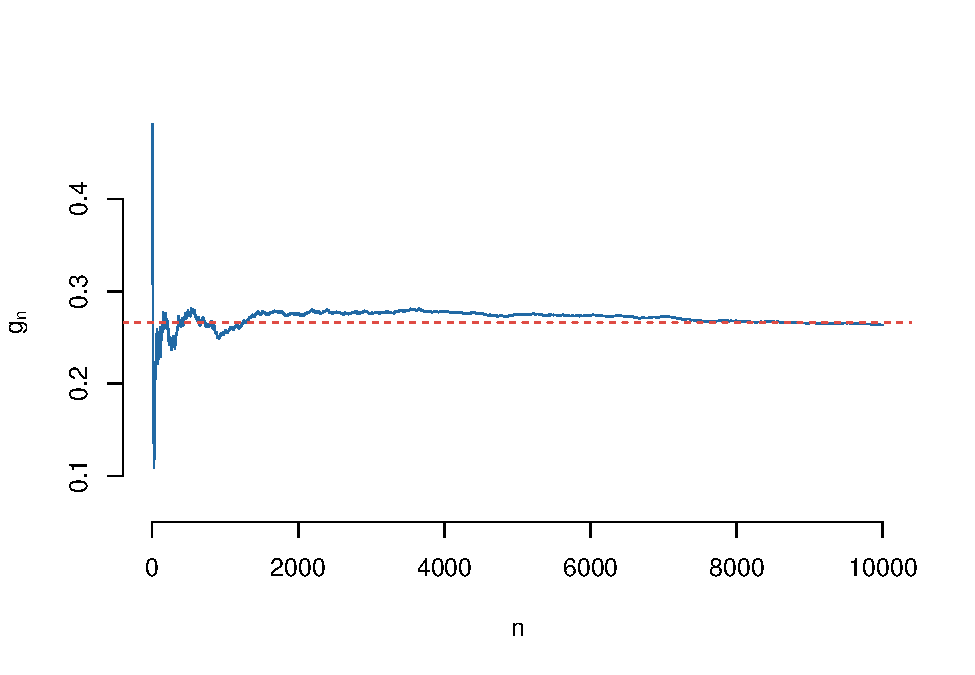
\includegraphics[width=0.8\linewidth]{Lab_3_files/figure-latex/unnamed-chunk-15-1} \end{center}


\end{document}
